\documentclass[11pt]{article}
\pdfoutput=1
\usepackage{jcappub}
\usepackage{aas_macros}
\usepackage{graphics,graphicx, url}
\usepackage{amsmath,amssymb}
\graphicspath{{figures/}}
\def \figwidth{0.9\textwidth}
\def \halffigwidth{0.45\textwidth}
\begin{document}

\title{Primordial Potential Reconstruction Constrained by a Measured Tensor Amplitude and the Preheating Regime}
\author[a]{J. Richard Bond}
\author[a,b]{Jonathan Braden}
\author[c]{Andrei Frolov}
\author[a]{Zhiqi Huang}
\author[d]{Pascal Vaudrevange}
\affiliation[a]{CITA}
\affiliation[b]{Dept. of Physics, U of T}
\affiliation[c]{Simon Fraser University}
\affiliation[d]{Germany}

\emailAdd{bond@cita.utoronto.ca}
\emailAdd{jbraden@cita.utoronto.ca}
\emailAdd{frolov@sfu.ca}
\emailAdd{zqhuang@cita.utoronto.ca}

\abstract{The shapes of the primordial scalar power spectra are the key quantities to unravel the physics of the inflationary epoch. Blahblah...}

\date{\today}
\maketitle

\section{Introduction}

The cosmic microwave background radiation is a unique window into the physics of energy scales above TeV. Progress towards harvesting its information content has been steady on the experimental side, starting with the COBE experiment \cite{COBE1996}, continuing with balloon borne experiments such as Boomerang \cite{Boomerang2001, Boomerang2003}, ground-based experiments such as ACT \cite{ACT2013, ACT2014}, SPT \cite{SPT2013, SPT2014} and BICEP \cite{BICEP2}, and the satellites WMAP \cite{WMAP9Maps, WMAP9Cosmology} and Planck \cite{Planck2013Overview, Planck2013PowerSpectra, Planck2013Parameters}. They delivered a picture of a universe that is extremely homogeneous: Gaussian fluctuations sit on top of a uniform background of photons that stream to us from the surface of last scattering at redshift about $1100$, with an amplitude of about $10^{-5}$. Decomposing this image of the microwave sky into spherical harmonics shows an angular power spectrum whose features are well understood. Acoustic oscillations in the primordial photon-baryon fluid freeze out at the surface of last scattering, with the photons streaming (almost) freely towards us, showing the familiar acoustic peaks in the angular power spectrum. Their locations and relative amplitudes allow us to infer the energy content of the universe.

While experimental advances have been formidable, the exact properties of microscopic theories responsible for the inflationary period remain elusive. A plethora of different scalar field potentials have been suggested, and many of them are compatible with current observations. From a theoretical perspective, the best that can be said is that there are many scalar fields in string theory. As for their potentials, not much is known. Even though some advances have been made in building models of inflation based on or inspired by string theory \cite{KKLT, Blanco-Pillado:2004ns, Blanco-Pillado:2006he, KKLMMT, CQ, GKP, Silverstein:2008sg}, the vast majority of the string landscape is still unchartered.


Traditionally the inflationary dynamics are described in the slow-roll approximation, assuming that the inflaton field rolls slowly (or with small acceleration) down its potential. For the simplest single-field slow-roll models, both the scalar and tensor power spectra are very close to power-law and the tilt of tensor power spectrum satisfies a consistency-relation. As a consequence, as far as only observables are concerned, these models can be described with three parameters: the amplitude of the scalar power spectrum ($A_s$), the tilt of the scalar power spectrum ($n_s-1$), and the tensor-to-scalar ratio ($r \equiv A_T/A_s$ where $A_T$ is the amplitude of tensor power spectrum). The tilt of the tensor power spectrum, according to slow-roll approximation, is $n_t = -r/8$. 


Thanks to the plethora of observational data that are already available today, we can go beyond the simplest models and ask whether a single-field slow-roll model is adequate to describe the data. To answer such a question it is necessary to extend the parameter space with reasonable theoretical motivations. For a broad class of models, the tensor power spectrum remains to be a power-law with a small tilt. This is because the tensor power spectrum, almost model-independently, only depends on the energy scale of inflation, which by definition does not vary much. Observationally, because of the smallness of $B$-mode polarization signature and the limited range of scales where tensor power spectrum can be measured, it is very difficult to measure features in the tensor power spectrum. Thus, it is reasonable to keep the parametrization of tensor power spectrum unchanged. For the future, we might be able to explore the small tilt of tensor power spectrum and test the sinlg-field slow-roll consistency relation. In that case, $n_t$ should be introduced as a free parameter. For the current data, we do not bother to do so as $n_t$ at this stage is far from being measurable to the accuracy of testing the consistency relation. However, while a broader class of inflation models are permitted, the scalar power spectrum, becomes very model-dependent \cite{Linde1996, Starobinsky1998, Lyth2003, Barnaby2009b, Bond2009}. Phenomenologically, back to the early COBE era, a running parameter $n_{\rm run}$ was already introduced as a minimal extension to describe the scale dependence of the tilt of scalar power spectrum \cite{Kosowsky1995}. Theoretically, a tiny running $\lesssim 10^{-3}$ is expected from  single-field slow-roll models. A detectable running $\gtrsim 0.01$ requires a very slow phase-transition over many efolds of inflation, which is not very well motivated. However, if only one or two degrees of freedom are to be added, there is no ``optimal'' or ``universal'' parameterization that can describe a much broader class of models. For this reason, the running parameter remains to be ``the standard extension'' to date. This situation, however, can be changed if we add more degrees of freedom into the parametrization. Because the observable range of cosmological scales is about ten efolds, a function interpolated from about 10 knots can cover most of the features that are not much shaper than one efold in scale. This interpolation method, to be thoroughly explored in this paper, provides an alternative approach to study the primordial power spectra with very little theoretical priors imposed. The philosophy here is to let the data guide our theoretical thoughts.

If we only consider the CMB temperature-temperature (TT) auto-correlation, the immediate problem of allowing an ``arbitrary'' shape of scalar power spectrum is that the tensor contribution to the TT correlation can be mimicked by a scalar power spectrum with a proper shape. There is hence a strong degeneracy between the scalar and tensor power spectra. The theoretical prediction of the amplitude of tensor power spectrum varies from $r\sim 10^{-10}$ for many string-motivated small-field models to  $r\sim 0.1$ for large-field models, with the scales in between almost all plausible. Thus, this degeneracy cannot be relieved by imposing a theoretical prior. We need additional data to constrain the tensor power spectrum independently. The recent detection of B-mode polarization in CMB \cite{BICEP2}, although remains to be confirmed by other experiments, casts a light on solving this problem.

This paper is structured as follows. Blahblah...

\section{Reconstructing Primordial Trajectories if the Tensor-to-Scalar is Measured}

\subsection{Scalar Curvature Power Spectrum }

Following the convention in the literarture we use $\Delta^2_{S}(k) = \frac{k^3P_S(k)}{2\pi^2}$ and $\Delta^2_T(k) \equiv \frac{k^3P_T(k)}{2\pi^2}$ to denote the scalar- and tensor power spectra, respectively. These power spectra are $k$-volumed weighed, and are nearly flat for most of the inflation models.

The CMB temperature-temperature angular power spectrum $C_\ell^{TT}$ from tensor contribution with $r=0.2$ (the central value suggested by BICEP2 \cite{BICEP2}) can be generated by an effective scalar power spectrum shown in Figure~\ref{fig:effps}. Planck best-fit cosmology is used \cite{Planck2013Parameters}.  To avoid this degeneracy between tensor- and scalar contributions, we can either assume $r$ to be some specific value and discuss the constraints on scalar power spectrum under such an assumption, or use BICEP2 data to independently constrain $r$. We will apply both approaches in this section. When fixing $r$ we use fiducial values $r=0.02$,  $0.2$ and $0.5$ as typical examples, whereas for ``free'' $r$ we use a flat prior $0\le r < 1$. The lower bound $r\ge 0$ is defined by theory, while the assumed upper bound $r<1$ does not affect the result as long as it is much higher than the observational upper bound, which, from BICEP2 is about $0.4$ at 99.7\% confidence level.   


\begin{figure}
  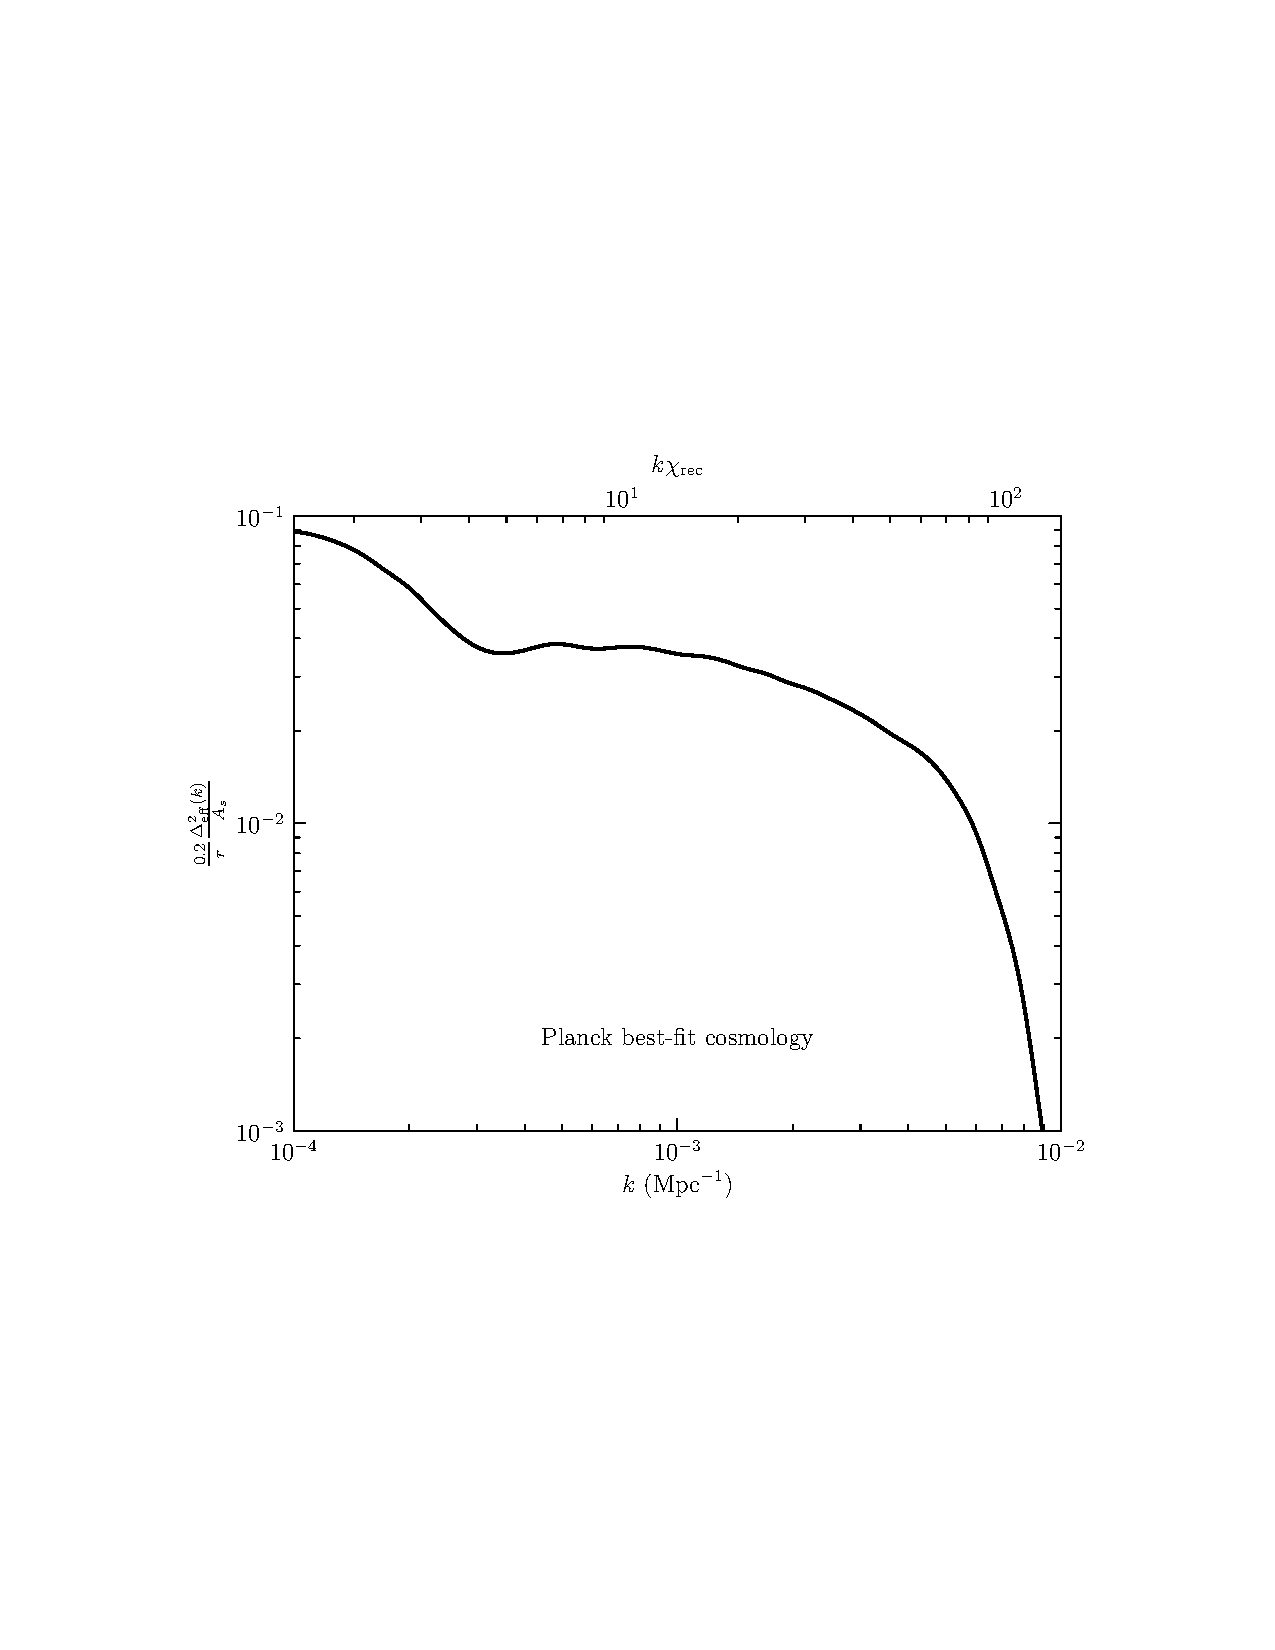
\includegraphics[width = \figwidth, trim = 1in 2.9in 1in 2.9in]{ten_eff_ps.pdf}
  \caption{The effective scalar power spectrum that produces the same $C_\ell^{TT}$ as $r=0.2$ tensor power spectrum would do. Planck best-fit cosmology is assumed. \label{fig:effps}}
\end{figure}


We use the public available software CosmoMC \cite{CosmoMC} to do Monte Carlo Markov Chain (MCMC) calculations. The software is modified to include our parametrization of the primordial power spectra. For the runs with fixed $r$, we use Planck data including lensing (Planck), WMAP polarization (WP), ACT and SPT high-ell data (highL) and Baryon Acoustic Oscillations (BAO) constraint from Sloan Digital Sky Survey (SDSS) \cite{SDSSDR9} and Six-degree-Field Galaxy Survey (6dF) \cite{Jones2004, Jones2009}. The BICEP2 data is used only for runs with $r$ varying. We use 11 knots as a representative case. We verify, by varying the number of knots (typically, from 9 to 15), that the results are not sensitive to the number of knots.

A $n$-knots parametrization is constructed by interpolating scalar power spectrum between $n$ knots. In our parametrization,  $A_s$ is still defined as the amplitude of scalar power sepctrum at $k_{\rm pivot}=0.05 {\rm Mpc}^{-1}$. The knots $k_1$, $k_2$, ..., $k_n$ are uniform in $\ln k$, with $k_{\rm pivot}$ being one of the knots $k_{i_p} = k_{\rm pivot}$ ($i_p$ is a fixed integer between $1$ and $n$). Additional $n-1$ parameters are introduced to describe the deviation from scale-invariance. They are defined as $\gamma_i\equiv \Delta^2_S(k_i)/ A_s$, for $i = 1, 2, \ldots, i_p - 1, i_p+1, \ldots, n$.  The choice of $i_p$ and spacing $\delta\ln k \equiv \ln (k_{i+1}/k_i)$ depends on the number of knots. The criterion is that the relevant cosmological scales (roughly from $10^{-4}{\rm Mpc}^{-1}$ to $0.2 {\rm Mpc}^{-1}$) are covered from $k_1$ to $k_n$. For the MCMC runs we assume flat prior on $\ln A_s$ and $\ln \gamma_i$ ($i\neq i_p$). For scales between $k_1$ and $k_n$, we cubic-spline interpolate $\ln (\Delta^2_S(k)/A_s)$ with natural boundary conditions (second derivatives vanish). Whereas for scales beyond, we simply assume $\Delta^2_S(k) = \Delta^2_S(k_1)$ for $k<k_1$ and $\Delta^2_S(k) = \Delta^2_S(k_n)$ for $k>k_n$. As for the tensor power spectrum, we use a parametrization $\Delta^2_T(k) = r A_s (k/k_{\rm pivot})^{n_t}$ with $n_t = -r/8$ enforced. Note that in the literature $r$ is often defined as the tensor-to-scalar ratio at $k=0.002 {\rm Mpc}^{-1}$, slightly different from the $r$ defined here. We do not adopt this convention because with our parametrization, the scalar power at $k=0.002 {\rm Mpc}^{-1}$ is poorly measured, whereas the conventional parametrization extrapolates the scalar power to all scales with a constant $n_s$.

In Fig~\ref{fig:traj_power} we show the reconstructed scalar power spectrum under different assumptions about $r$. A down-turning is more significant for larger $r$ (either put in by hand or constrained by additional data) at scales $k<0.01 {\rm Mpc}^{-1}$. As shown in Fig~\ref{fig:effps}, such a down-turning can cancel the tensor contribution to $C_\ell^{TT}$ so that the total theoretical $C_\ell^{TT}$ remains in good agreement with the data. This is clearly demonstrated in Fig~\ref{fig:traj_cltt} where the corresponding $C_\ell^{TT}$ trajectories are plotted for each case. While the reconstructed power spectra differ significantly between large and small $r$'s, the $C_\ell^{TT}$ trajectories remain similar.



\begin{figure}
  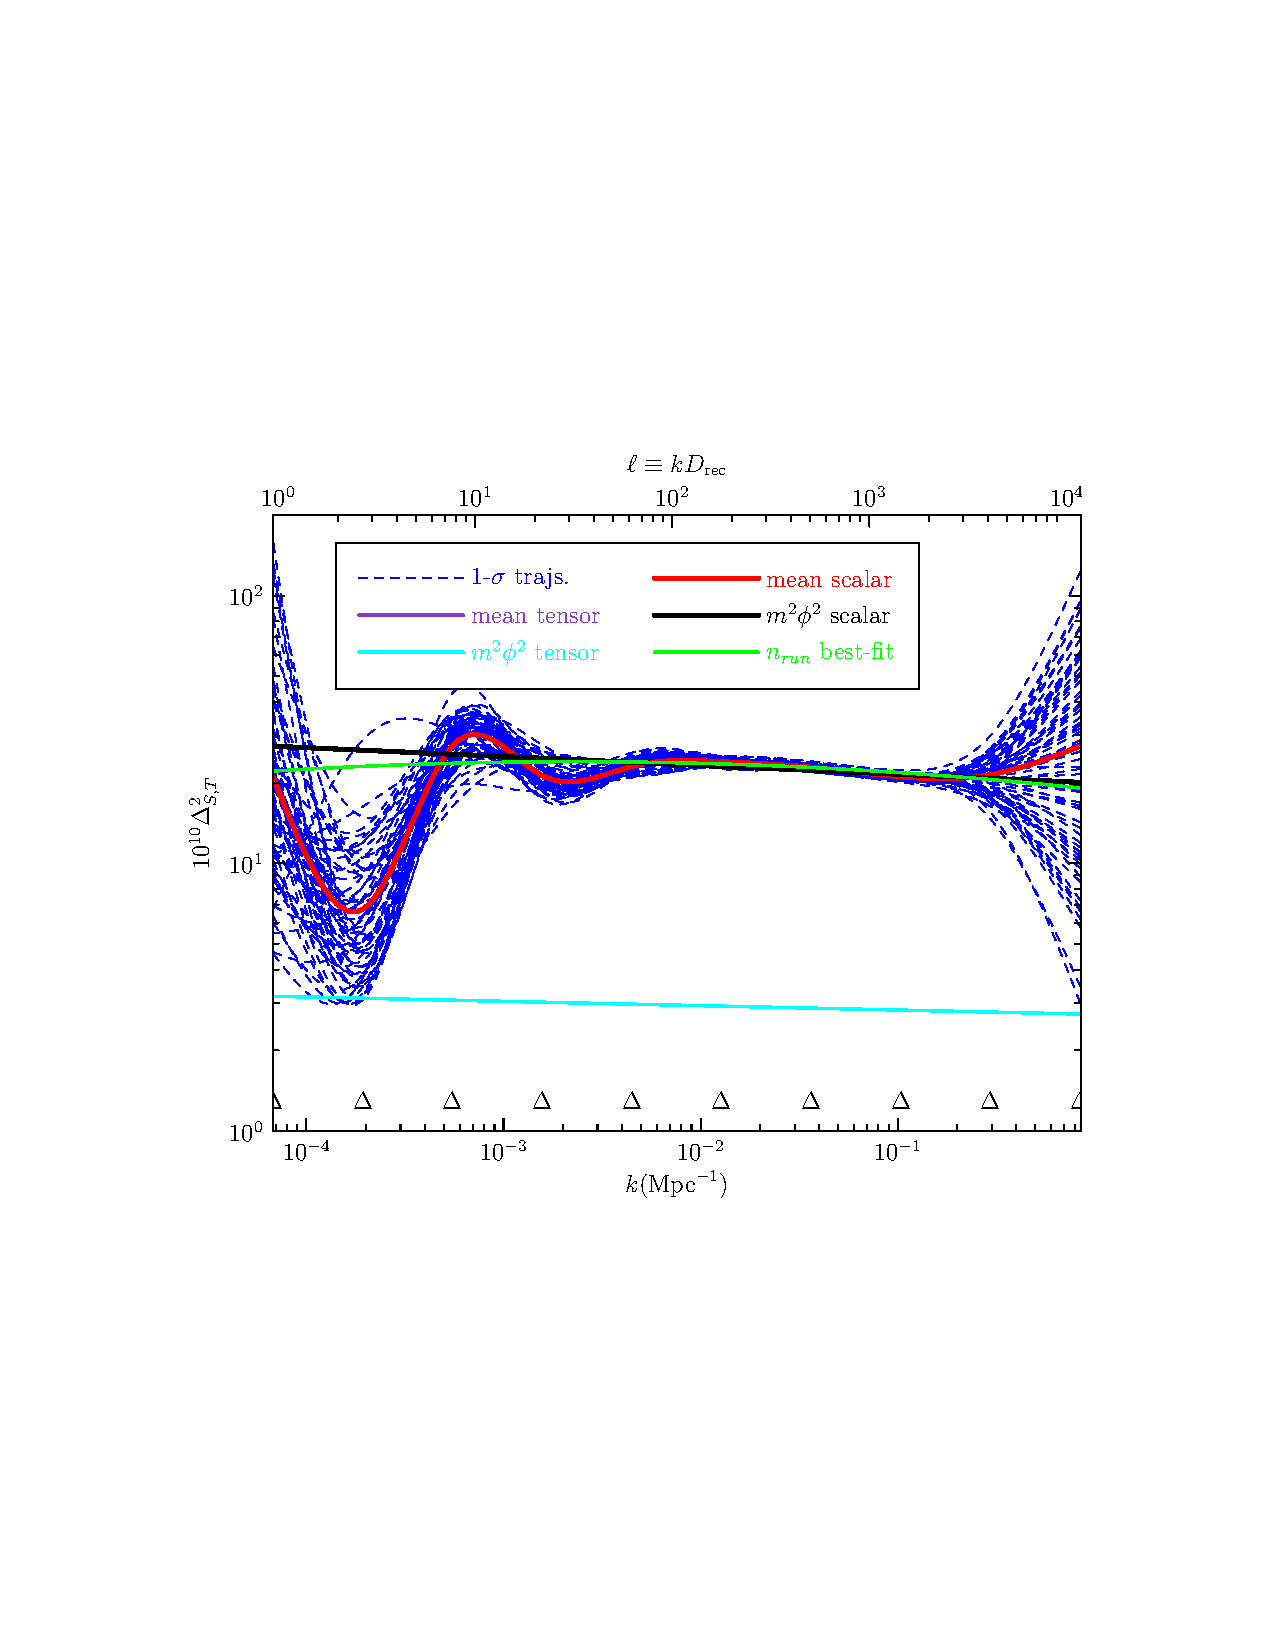
\includegraphics[width=\halffigwidth,  trim = 1in 2.9in 1in 2.9in]{nobicep_spline0_p11_r0d02_power_traj.pdf}% 
  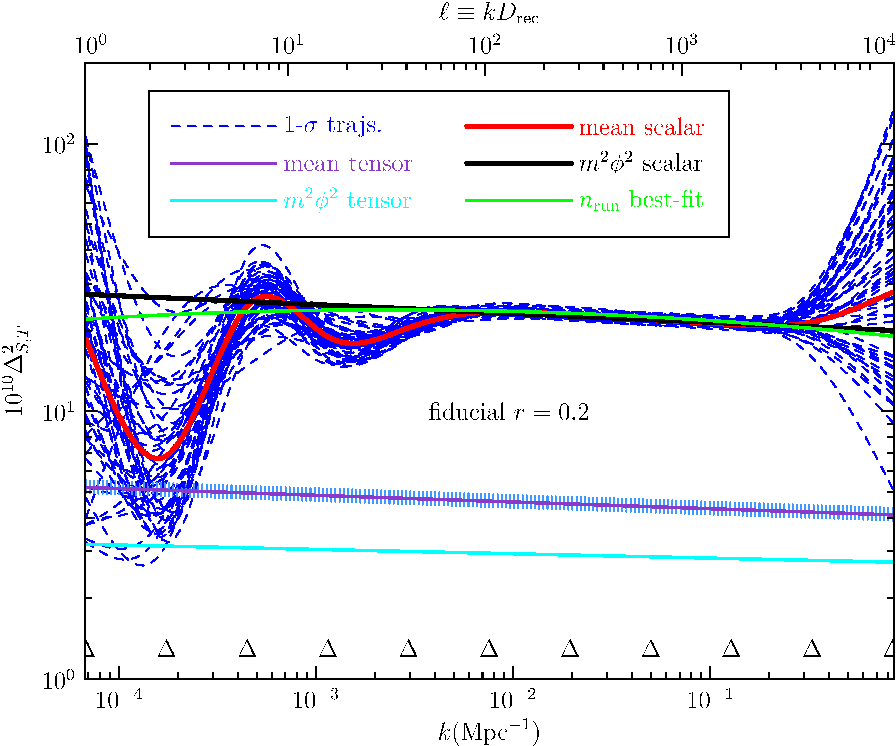
\includegraphics[width=\halffigwidth,  trim = 1in 2.9in 1in 2.9in]{nobicep_spline0_p11_r0d2_power_traj.pdf}
  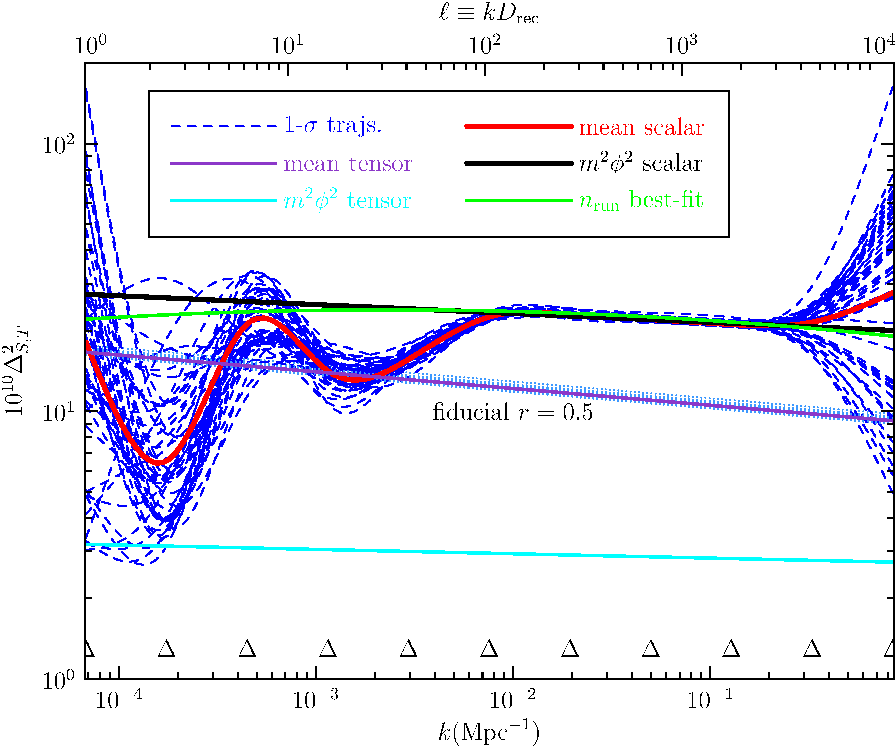
\includegraphics[width=\halffigwidth,  trim = 1in 2.9in 1in 2.9in]{nobicep_spline0_p11_r0d5_power_traj.pdf}%
  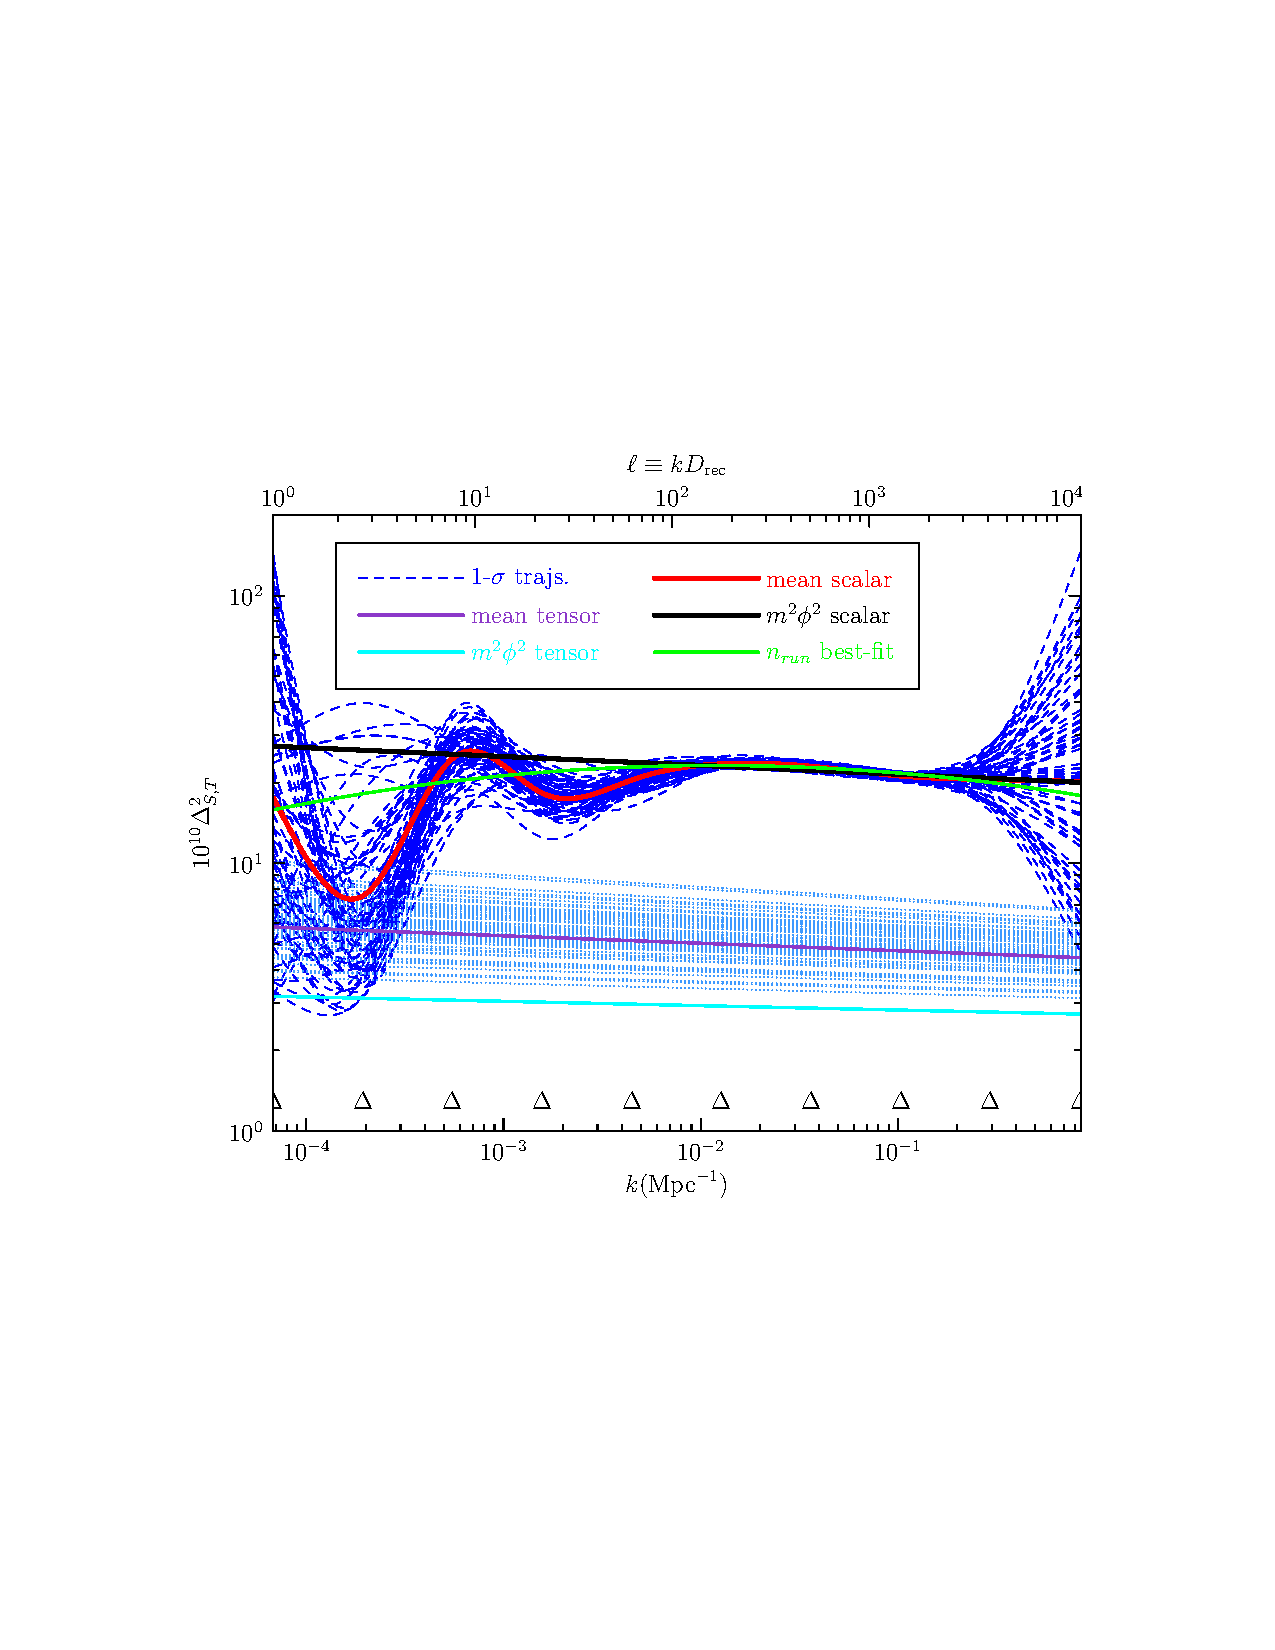
\includegraphics[width=\halffigwidth,  trim = 1in 2.9in 1in 2.9in]{spline0_p11_power_traj.pdf}
  \caption{The reconstructed power spectrum with $r = 0.02$, $r=0.2$, $r=0.5$ and free $r$ for top-left, top-right, bottom-left, bottom-right panels, respectively. The location of 11 knots used for interpolation are marked with $\Delta$ symbols. Data: Planck + highL + BAO. BICEP2 data is added in the free $r$ case. \label{fig:traj_power}}
\end{figure}



\begin{figure}
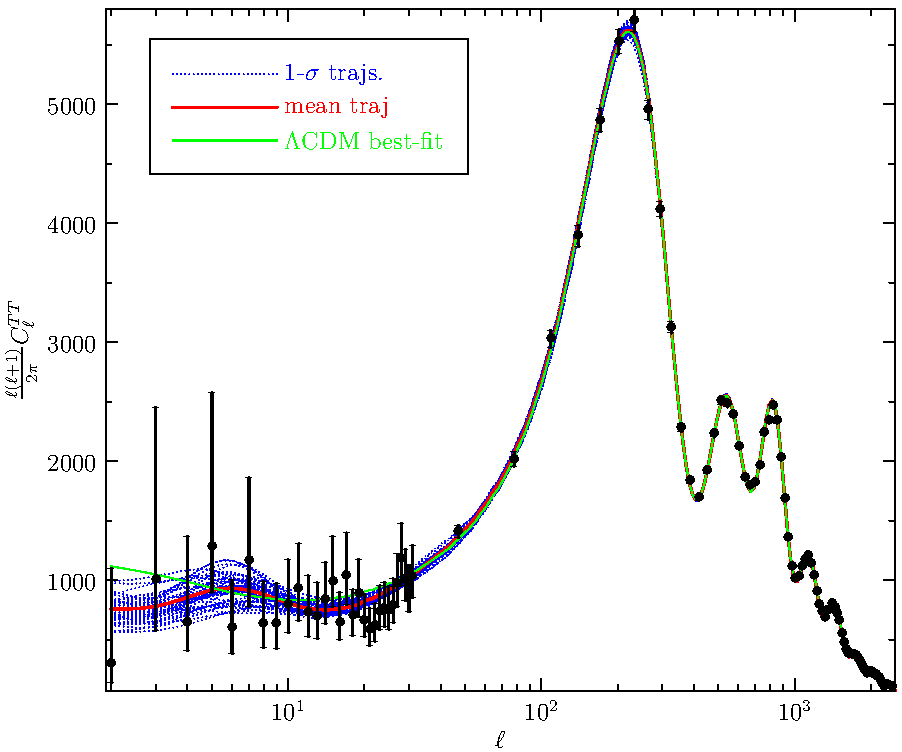
\includegraphics[width = \halffigwidth]{nobicep_spline0_p11_r0d02_clTT_trajs.pdf}%
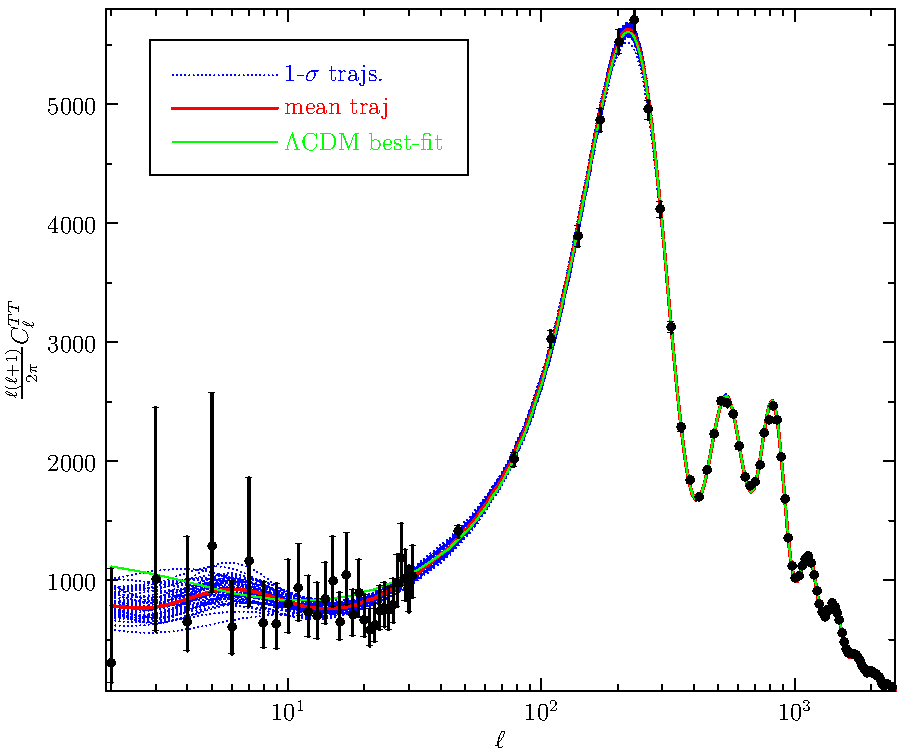
\includegraphics[width = \halffigwidth]{nobicep_spline0_p11_r0d2_clTT_trajs.pdf}
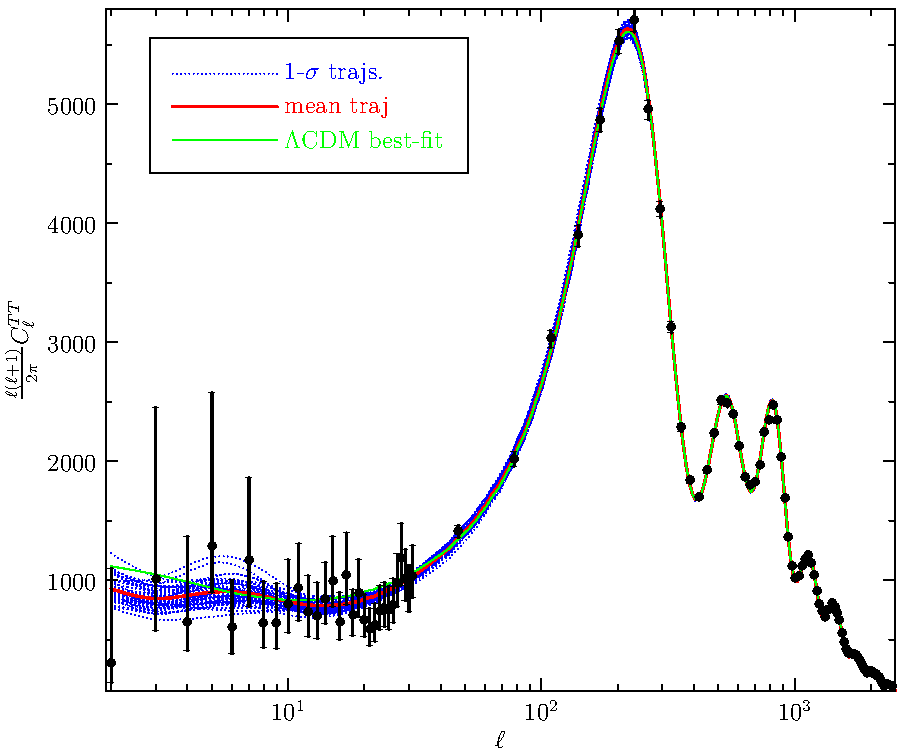
\includegraphics[width = \halffigwidth]{nobicep_spline0_p11_r0d5_clTT_trajs.pdf}%
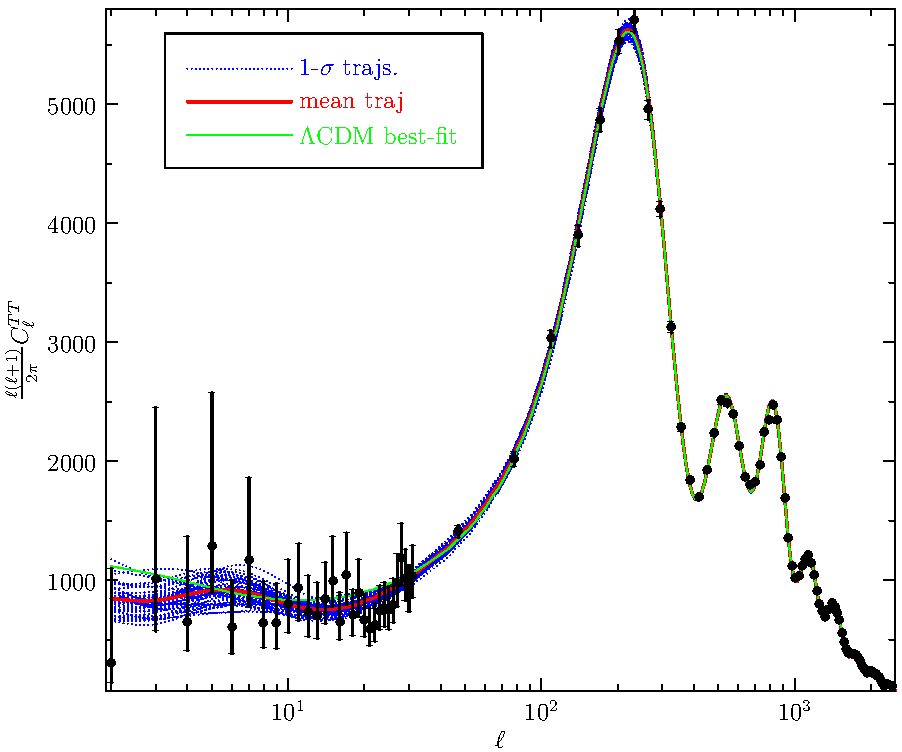
\includegraphics[width = \halffigwidth]{spline0_p11_clTT_trajs.pdf}
\caption{The reconstructed $C_\ell^{TT}$ trajectories for fiducial $r=0.02$ (left panel and $r=0.5$ (right panel). Data: Planck + WP + highL + BAO.\label{fig:traj_cltt}}
\end{figure}



\subsection{Acceleration Histories}

\begin{figure}
  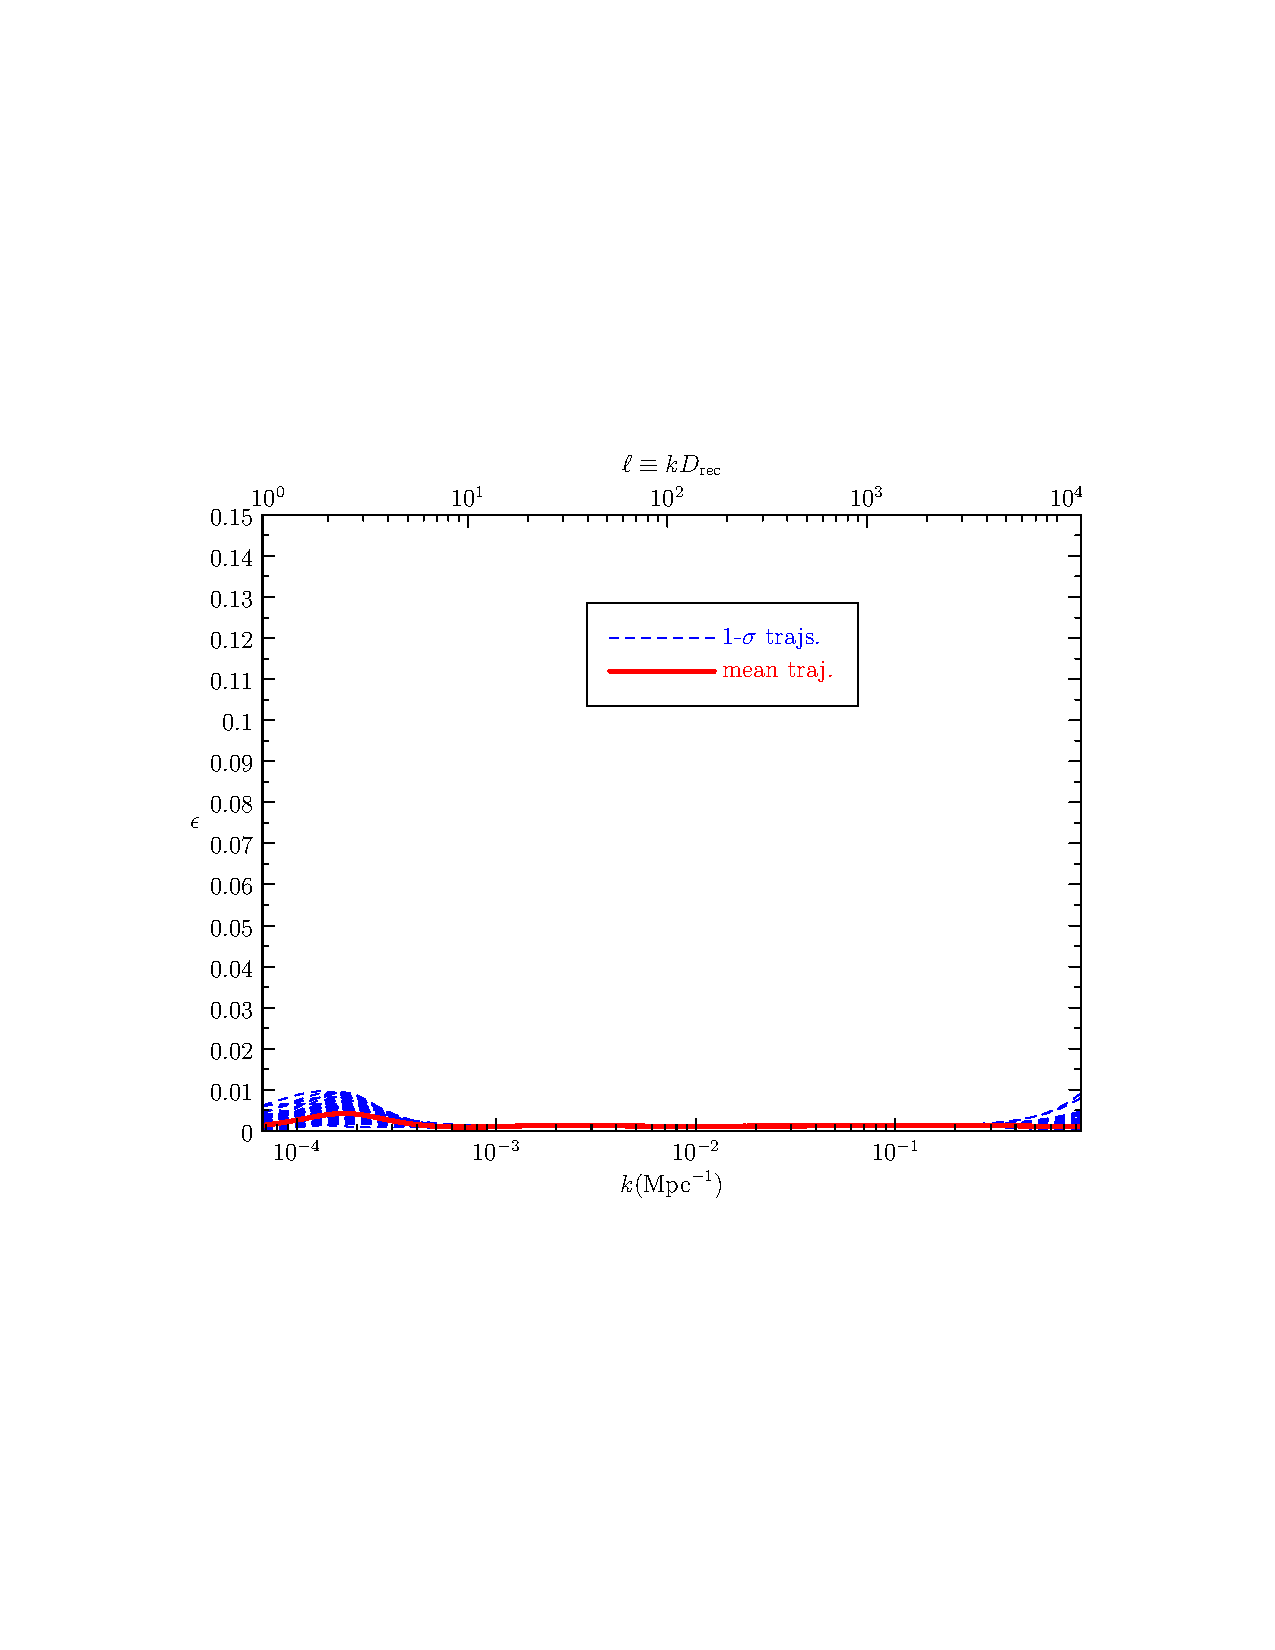
\includegraphics[width=\halffigwidth,  trim = 1in 2.9in 1in 2.9in]{nobicep_spline0_p11_r0d02_eps_traj.pdf}% 
  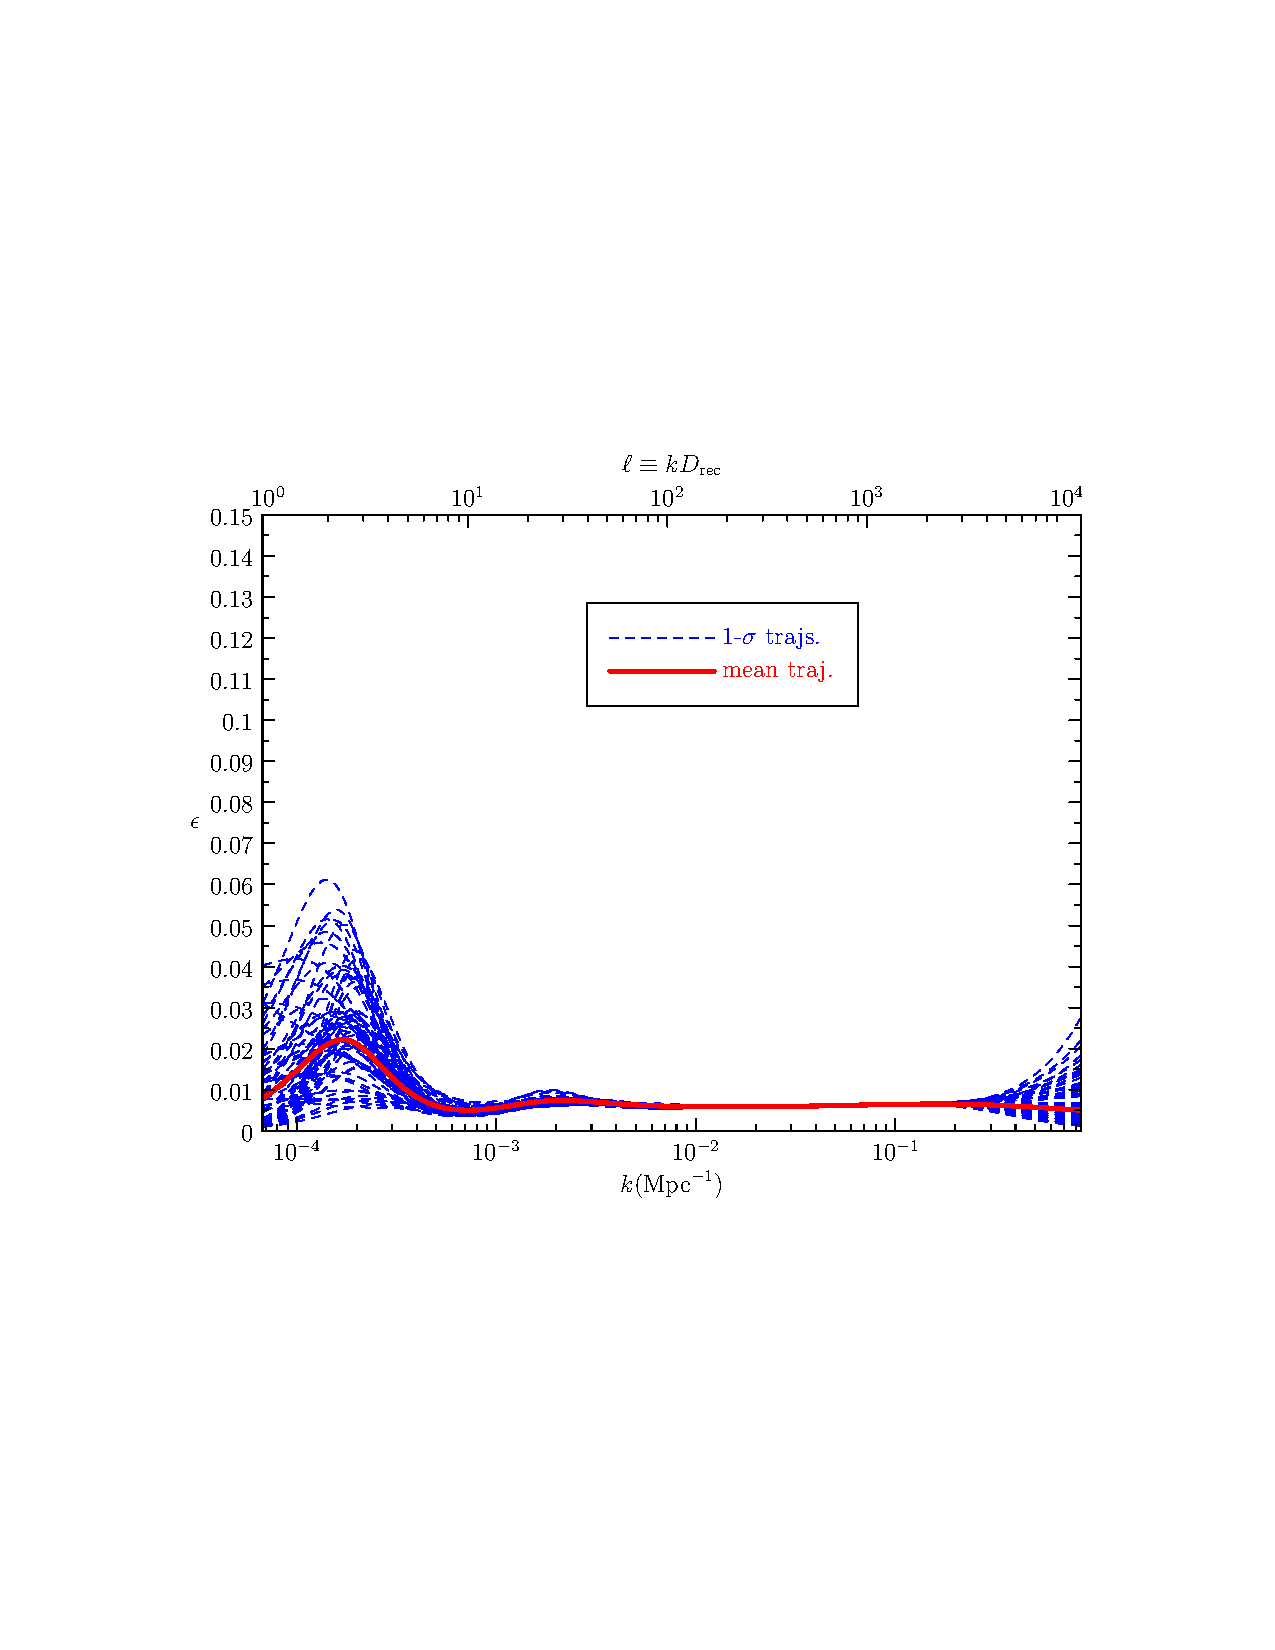
\includegraphics[width=\halffigwidth,  trim = 1in 2.9in 1in 2.9in]{nobicep_spline0_p11_r0d1_eps_traj.pdf}
  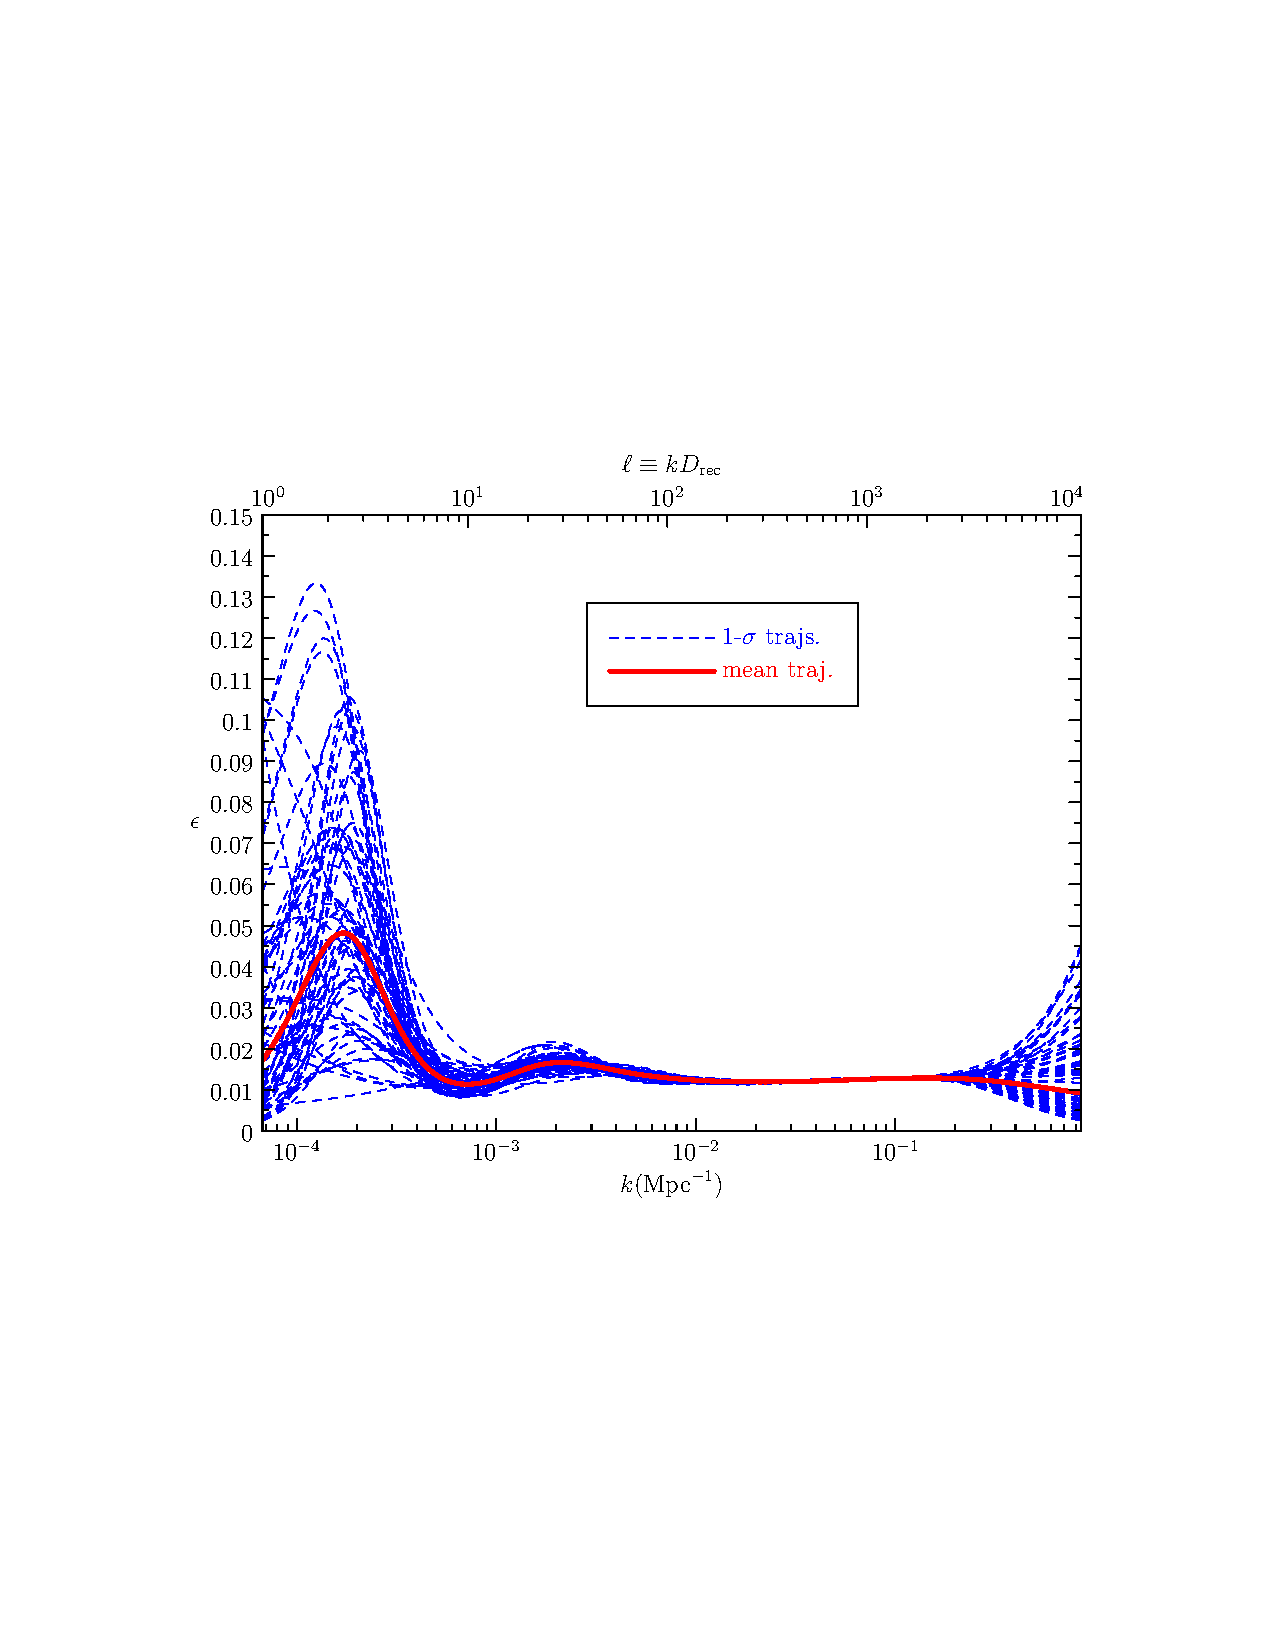
\includegraphics[width=\halffigwidth,  trim = 1in 2.9in 1in 2.9in]{nobicep_spline0_p11_r0d2_eps_traj.pdf}%
  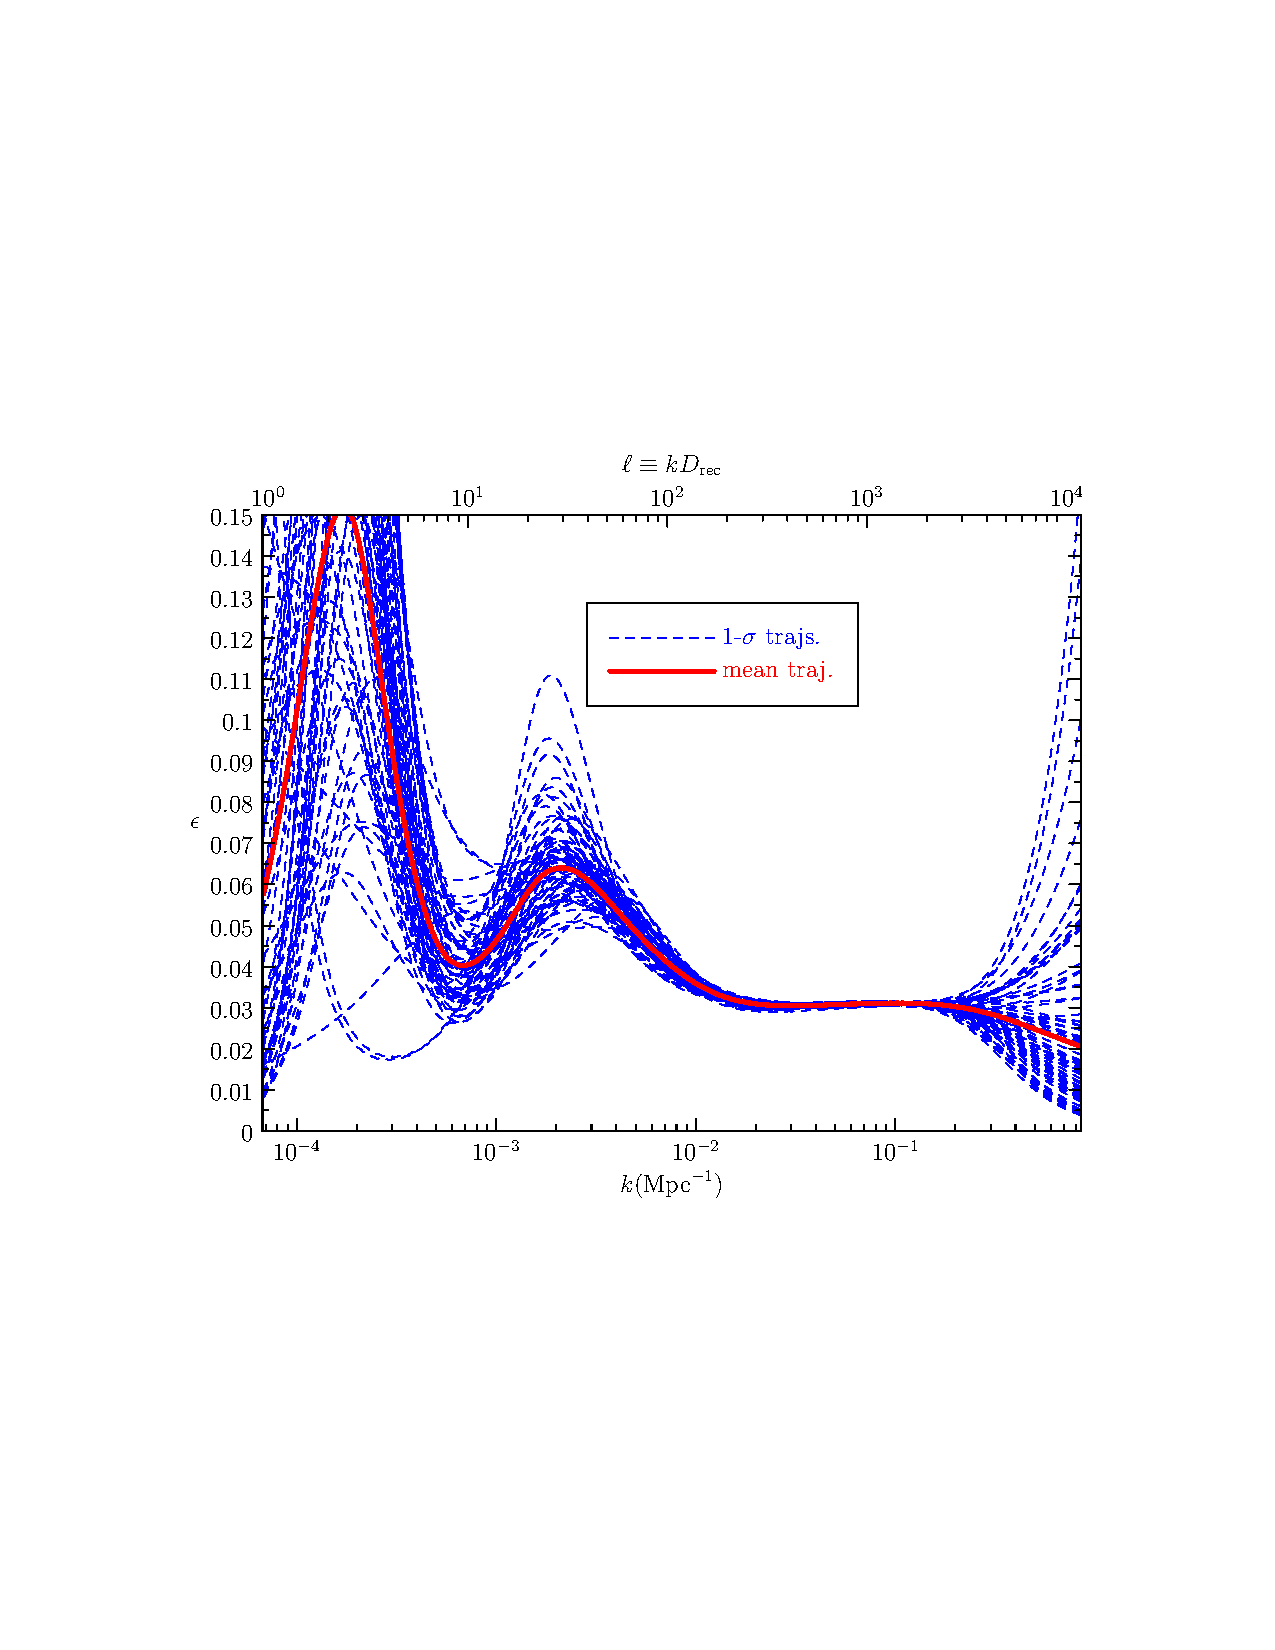
\includegraphics[width=\halffigwidth,  trim = 1in 2.9in 1in 2.9in]{nobicep_spline0_p11_r0d5_eps_traj.pdf}
  \caption{The reconstructed $\epsilon$ trajectories with fixed fiducial $r = 0.02$, $r=0.2$, $r=0.5$ for top-left, top-right, bottom-left, bottom-right panels, respectively. The location of 11 knots used for interpolation are marked with $\Delta$ symbol. Data: Planck + WP + highL + BAO. \label{fig:traj_eps_fixr}}
\end{figure}


\subsection{Inflaton Potential Reconstructions}

\begin{figure}
  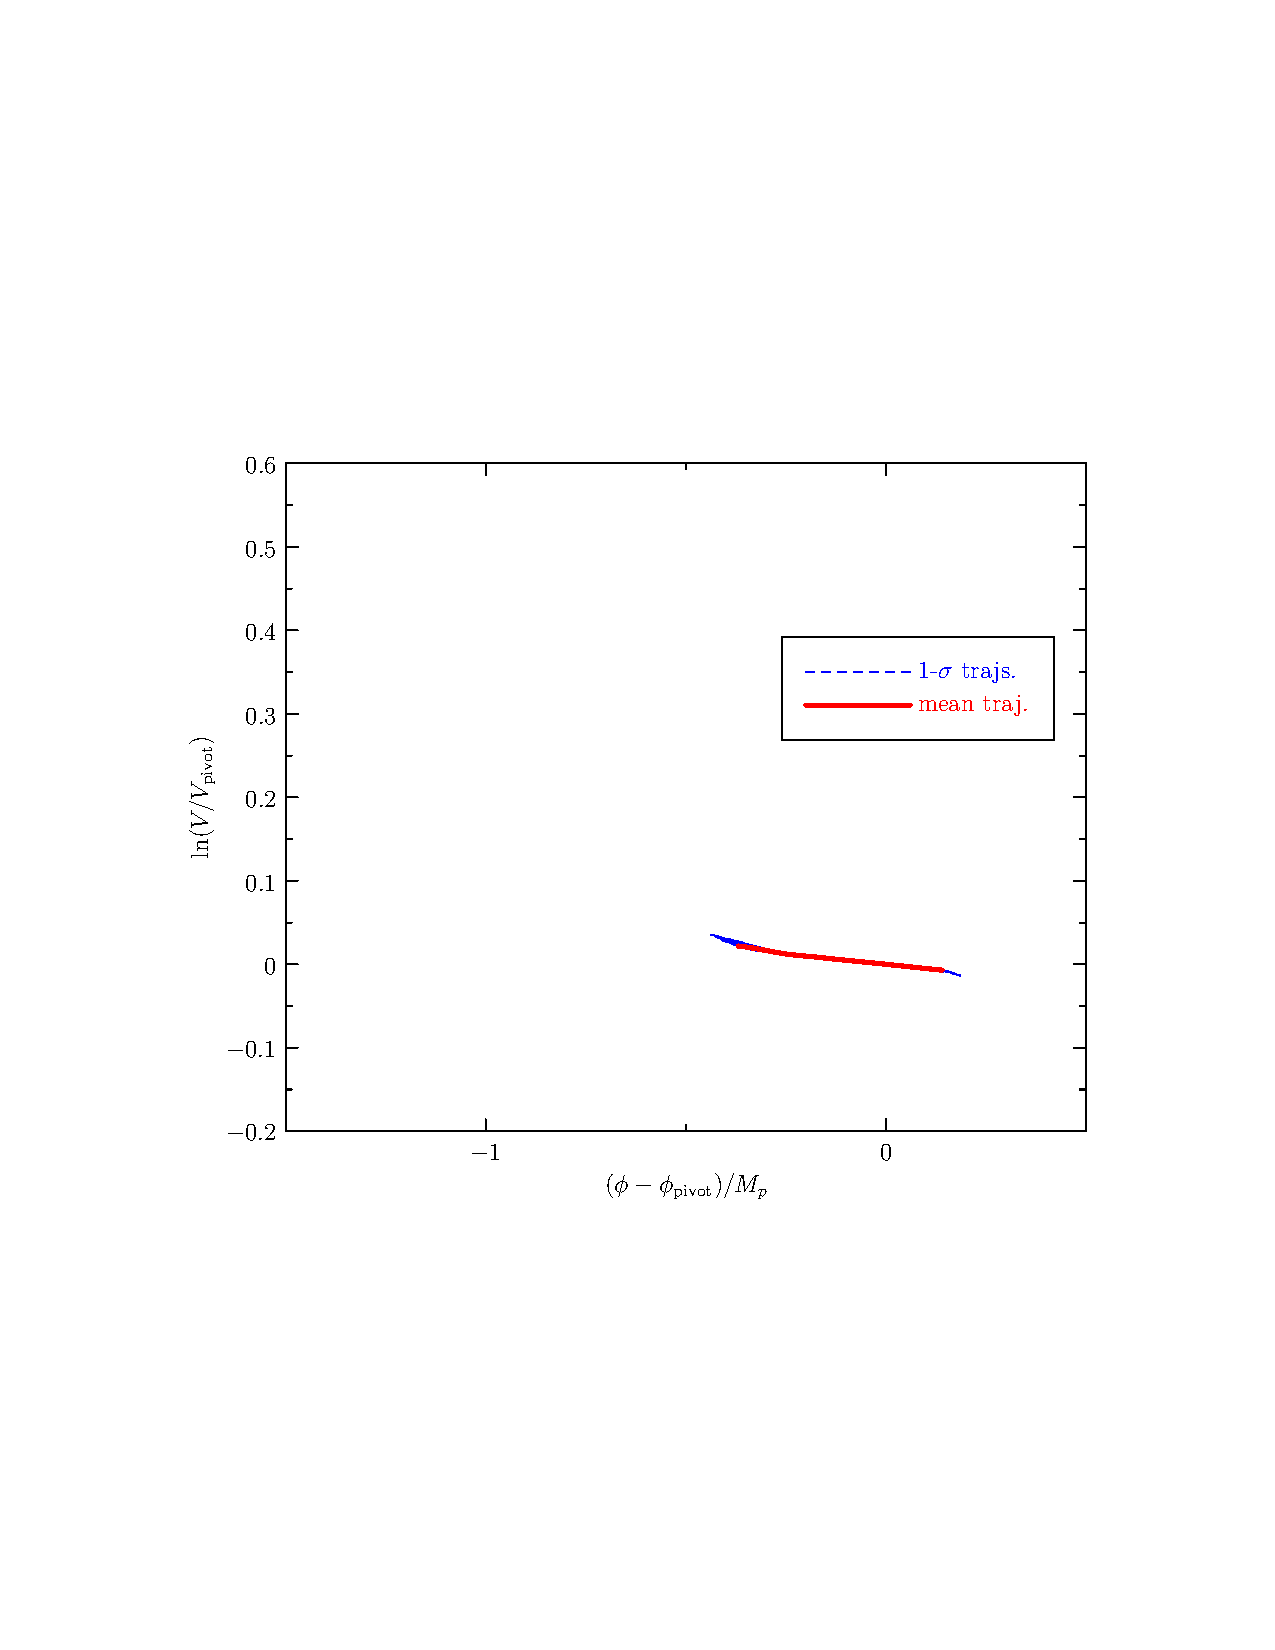
\includegraphics[width=\halffigwidth,  trim = 1in 2.9in 1in 2.9in]{nobicep_spline0_p11_r0d02_potential_traj.pdf}% 
  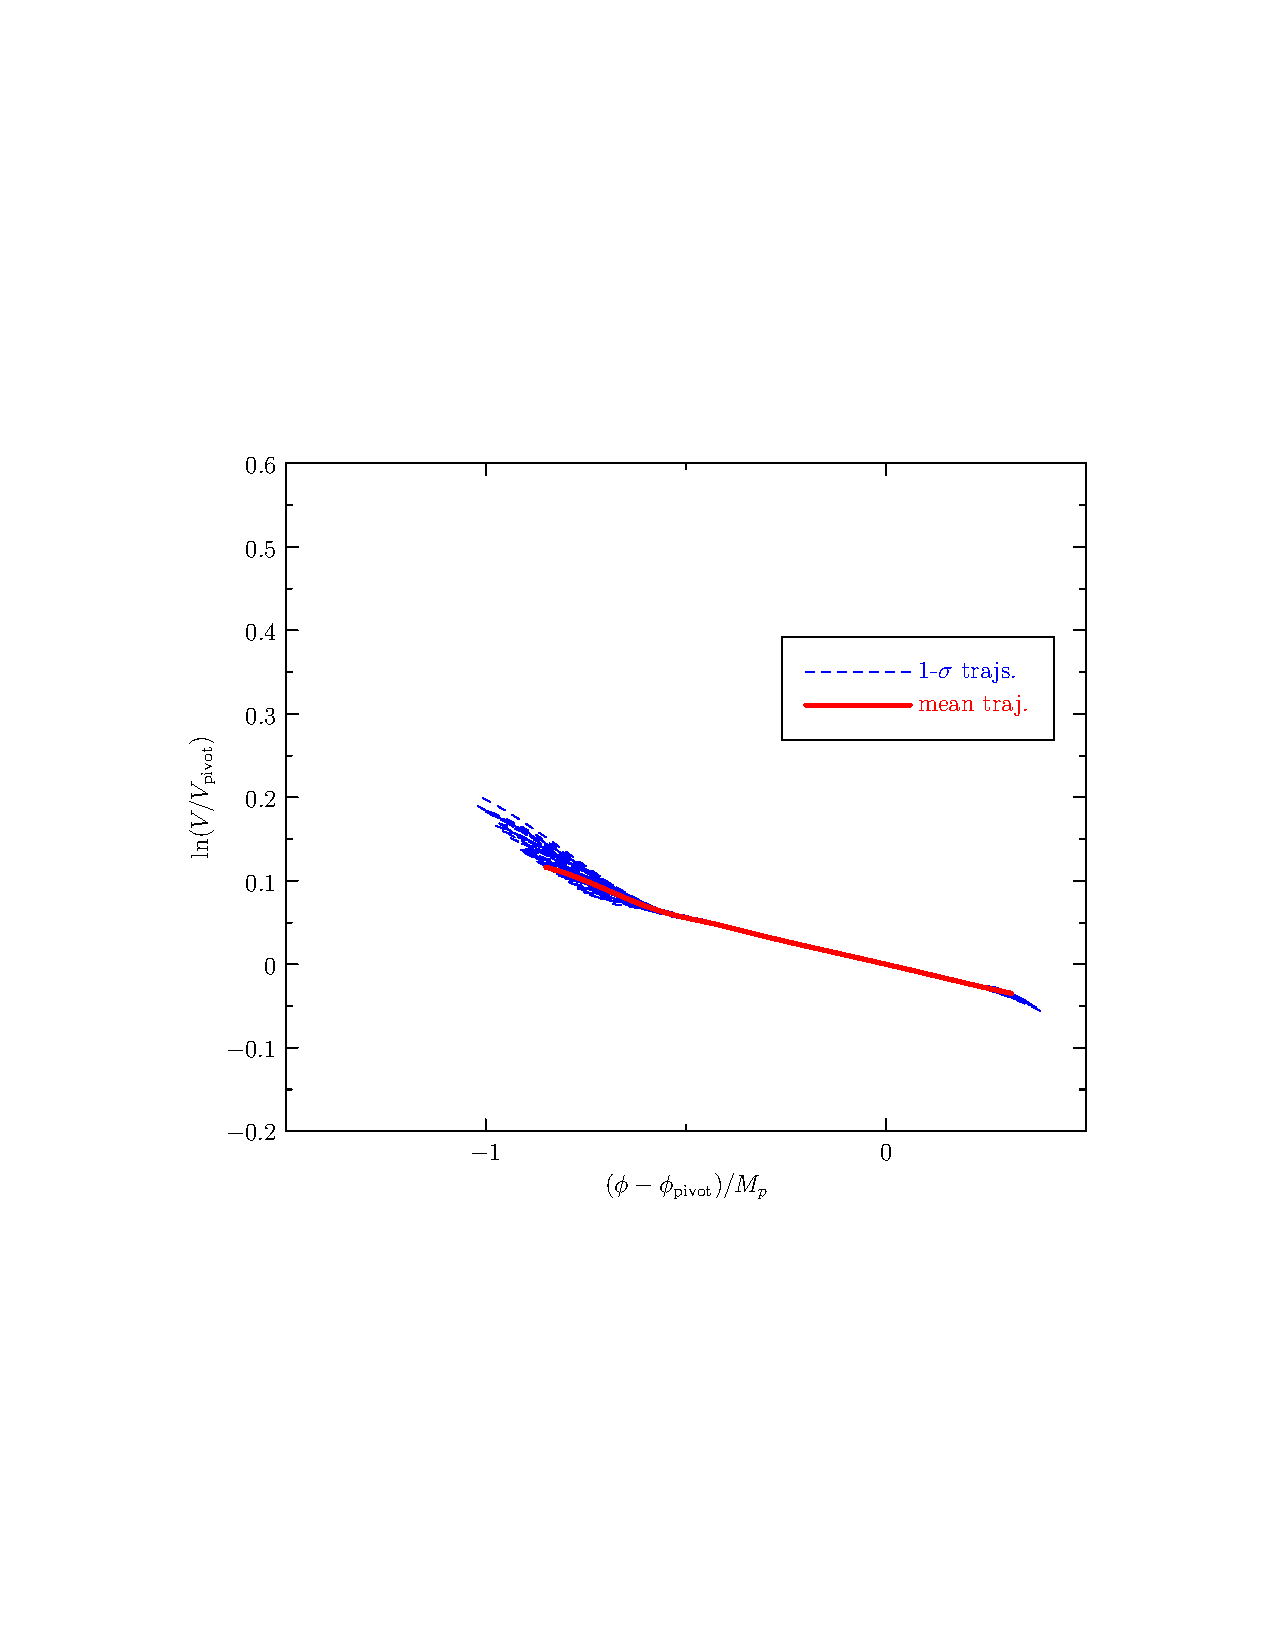
\includegraphics[width=\halffigwidth,  trim = 1in 2.9in 1in 2.9in]{nobicep_spline0_p11_r0d1_potential_traj.pdf}
  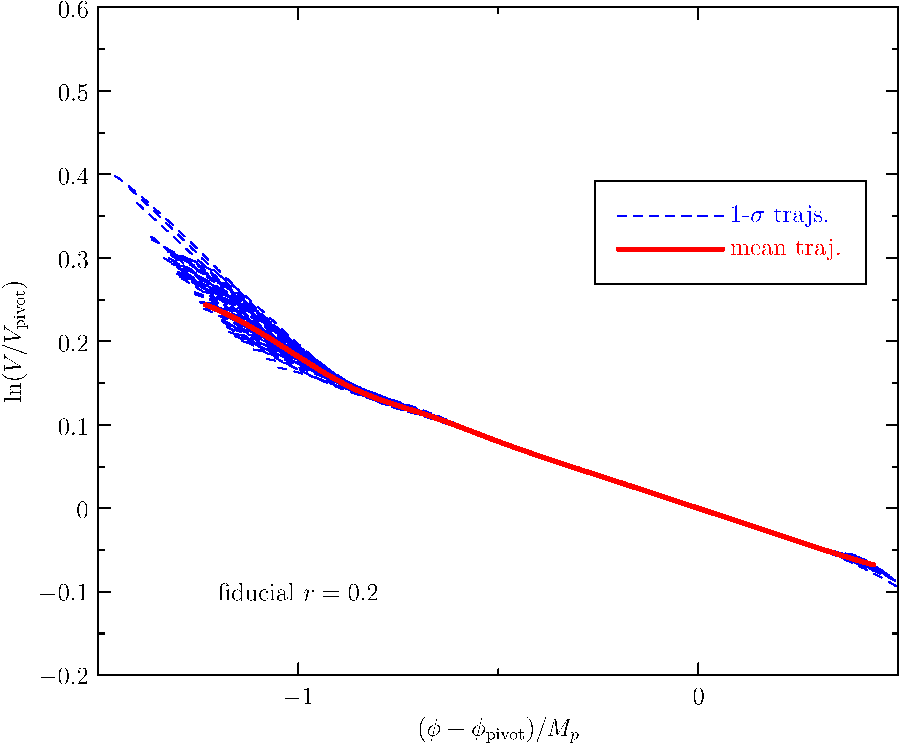
\includegraphics[width=\halffigwidth,  trim = 1in 2.9in 1in 2.9in]{nobicep_spline0_p11_r0d2_potential_traj.pdf}%
  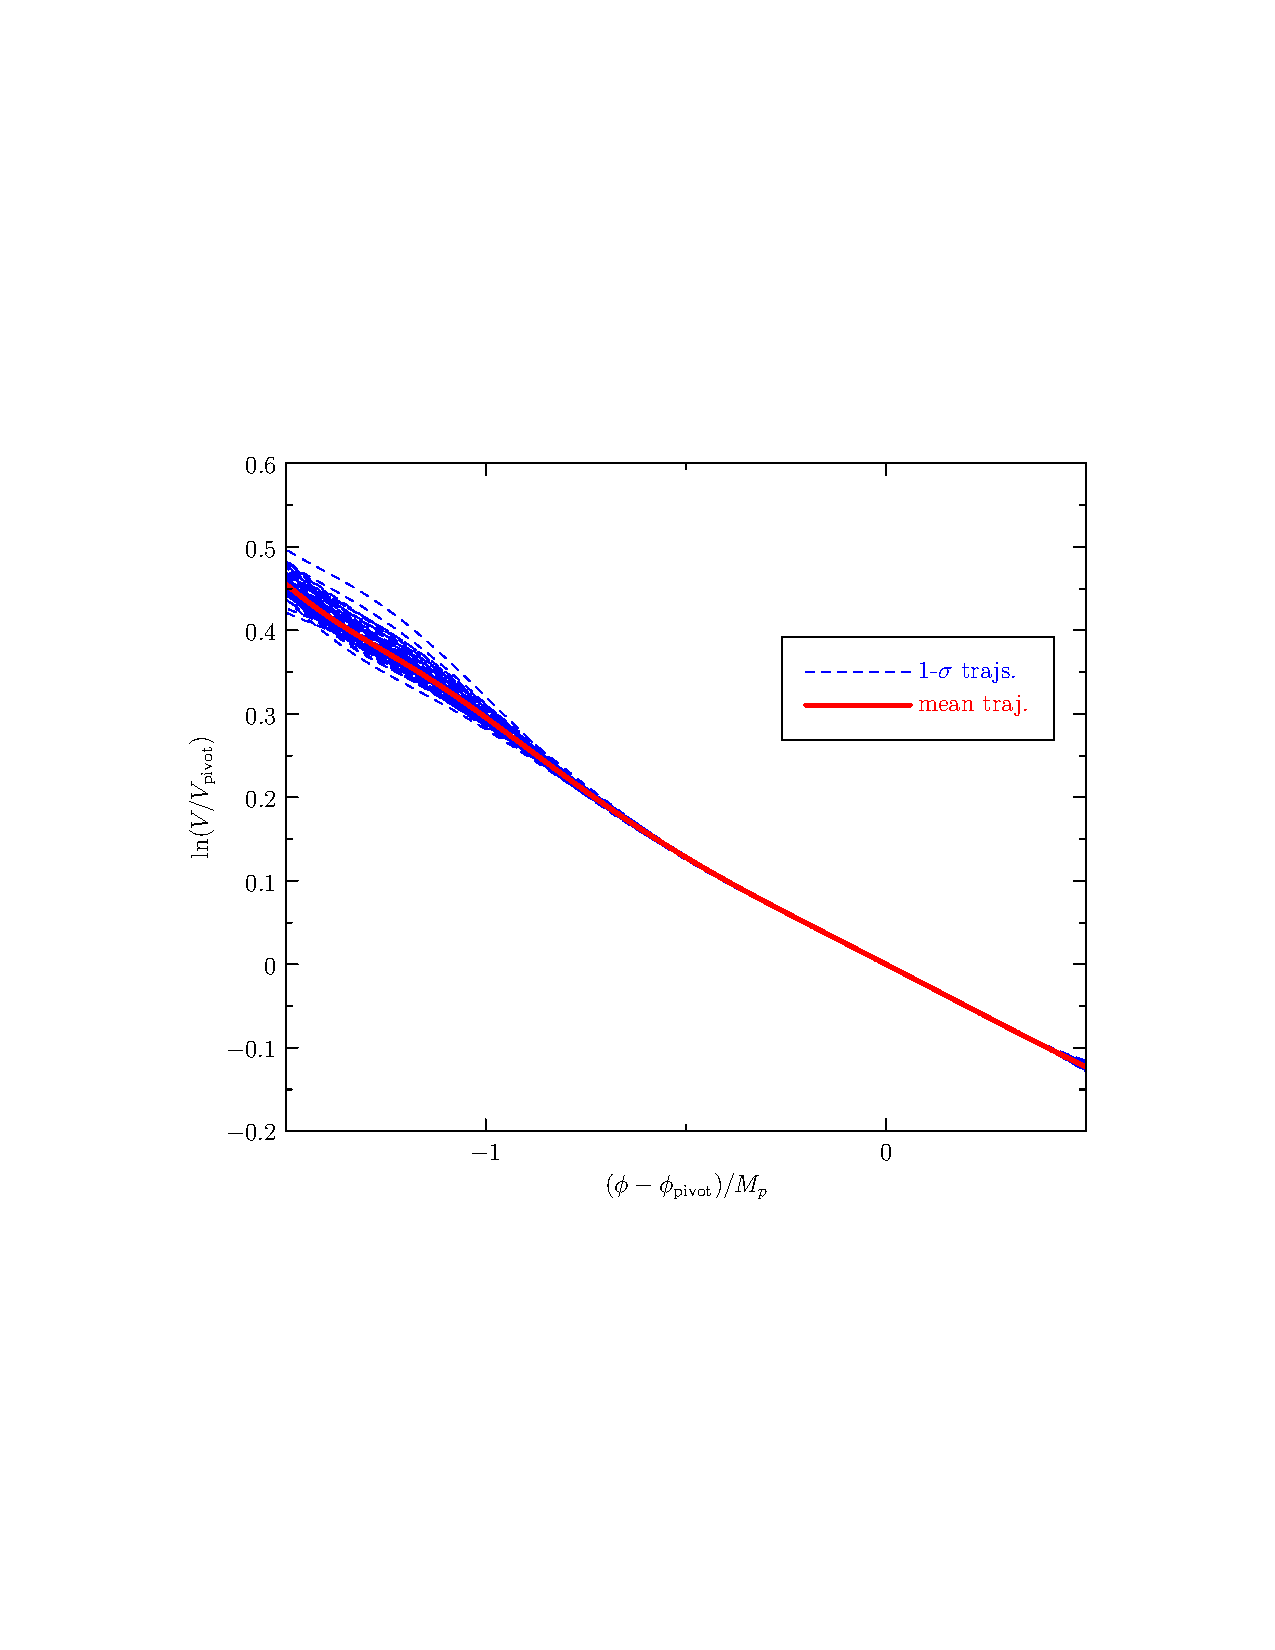
\includegraphics[width=\halffigwidth,  trim = 1in 2.9in 1in 2.9in]{nobicep_spline0_p11_r0d5_potential_traj.pdf}
  \caption{The reconstructed single-field potentials with fixed fiducial $r = 0.02,\ 0.1,\ 0.2,\ 0.5$ for top-left, top-right, bottom-left, bottom-right panels, respectively. The location of 11 knots used for interpolation are marked with $\Delta$ symbol. Data: Planck + WP + highL + BAO. \label{fig:traj_potential_fixr}}
\end{figure}


\section{Connecting Constrained Potentials in the Observable Range to the Potential in the Heating Regime }

B-modes help to really nail down the form of the potential during the
inflationary phase.  
Unfortunately, without a precise model to consider, the inflationary
dynamics are effectively independent of the reheating dynamics.
In particular, the inflaton condensate can break up via a variety of
different mechanisms depending on the ``shape'' of the potential
(tachyonic/spinodal instability, perturbative decay, amplification of
additional fields via parametric resonance followed by rescattering,...). 
The question is then how to relate the inflationary potential to the
potential at the minimum that is relevant for (p)reheating.
This seems rather difficult in the general case, since the ``shape'' of the
potential could change rather dramatically between inflation and
post-inflationary oscillations.  As some examples, in the single field case
the potential could be flattened (or steepened) at large field values, or
there could be a waterfall transition to end inflation.  This allows for a
large hierarchy between the effective mass of the inflaton during inflation
and the effective mass of the field as it oscillates.  Therefore, in the
completely general case it seems unlikely that the inflationary dynamics
could tell us much about the preheating dynamics.

Roughly, we want to have $P(\{a_i\},\{b_i\}|r)$ (or perhaps
$P(\{a_i\}|\{b_i\},r)$ for the case that the inflationary part is well
constrained)
where the $a_i$'s are some parameters that characterize the minimum of the
potential, and the $b_i$'s characterize the inflationary part of the
potential.
One possible approach is simply to expand the potential in a Taylor series
around the minimum (including several fields not just the inflaton).
It might also be interesting to expand in some other set of basis functions
(Chebychev's, Rational Chebyshev's, etc.).
This would at least give a definite way to define the coefficients in the
expansion.

One very unsophisticated take on this would be that a large value of $r$
means we have some sort of large-field model of inflation (even $m^2\phi^2$
for example).
If something like a simple polynomial is a good fit to the data during
inflation, then it is not unreasonable to consider the implications of
simply using a Taylor expansion around the minimum of the potential for the
preheating as well as the inflationary dynamics.
Naively, I would say this puts us into preheating regime that is described
by the billiard picture (although this might not be true).
Since we have a large field model, the effective couplings of the inflaton
to other fields will be enhanced by $(\phi_{end}/m_{eff})^{power} \sim
(M_P/m_{eff})^{power}$ and the couplings in the model will have to be very
small to be in the perturbative regime.
If this is true, then preheating and the eventual development of
nonlinearly interacting inhomogeneous fields is the correct description of
the end of inflation (modelling with some simple decay models isn't), which
is of course exactly what we've been working on.

The cleanest way to connect the B-mode results to preheating would be to
just assume that the Higgs is the inflaton (assuming that some appropriate
non-minimal terms in the Lagrangian or quantum effects allow it to match
the data).
Then we at least know all of the interactions as the Higgs is oscillating
around its minimum (and there are couplings to the gauge bosons of the form
$g^2h^2Z^2$ so it is not that dissimilar from $\lambda\phi^4 +
g^2\phi^2\chi^2$ billiards.
There are a couple papers on Higgs preheating (0812.4624 and 0812.3622),
but no lattice/nonlinear analysis that I know of.
Of course, having isocurvature modes in the gauge fields is probably
severely constrained so this might not be that interesting, and dealing
with the fermions is nontrivial.


\section{Flattening Preheating Potentials via Conformal Transformations}

\begin{equation} V(\phi, \chi) = 1/4 \lambda \phi^4  - 1/2 \xi \phi^2 R  1/2 g^2 \phi^2 \chi^2 \, .
\end{equation}

Conformal V-flattening as in SBB89, explored there as Higgs inflation with variable Planck mass models. 

The kinetic piece transforms as 

The field going into canonical form is 

The potential is transformed  as 

SBB considered large $\xi$. 

This story was recently picked up by Kallosh and Linde, who considered $\xi = 1/6 -\Delta$, where $\Delta$ is small. 

This should be compared with the heavy field V-flattening described in Dong, Horn, Silverstein, Westphal 2011, with $\phi^{2n}, \ n<1$ 
via heavy field trough driving light inflaton $V_{eff}$ yielding 
$r = 8n/(N_I +n/3) 1-ns  = (n+1)/(N_I-n/6)$, as in bh95. These forms are P13 OK

An example is one of the first  monodromy cases considered, SW08, with $p=1/3$. Later the form adopted in  MSW08 had $p=1/2$ and a $ \cos $ term associated with a shift symmetry. Another example is  roulette inflation (Kahler moduli) BKKV, where V-flat appears naturally. 
 
\begin{figure}
\includegraphics[width=0.5\linewidth]{{{potseq-1}}}
\caption{Conformally transformed potentials $U(\psi )$ for a sequence of $\xi$, with $\lambda$ fixed. }
\end{figure}

\begin{figure}
\includegraphics[width=0.5\linewidth]{{{potseq-2}}}
\caption{Conformally transformed potentials for a sequence of $\xi$, with $\lambda/\xi^2$ fixed. }
\end{figure}

\begin{figure}
\includegraphics[width=0.5\linewidth]{{{af_phase_portrait_ximinus1_shading_N_phi_pi}}}
\caption{Phase portrait for the class of conformally flattened potentials considered here, with $\xi = -1$. The shading denotes $\ln a (\phi ,\pi_\phi )$. }
\end{figure}

\section{Caustics from Ballistic Trajectories}

Development of caustics in ballistic trajectories for
\begin{equation}
  \mathcal{L} = \frac{R}{2} - \frac{1}{2}\partial_\mu\phi\partial^\mu\phi - \frac{1}{2}\partial_{\mu}\chi\partial^{\mu}\chi + \xi\phi^2R - \frac{g^2}{2}\phi^2\chi^2
\end{equation}
{\bf Double check normalizations and coupling constant definitions}

\begin{figure}
\includegraphics[width=0.5\linewidth]{{{mom_zeta0.5}}}
\caption{Development of caustics for $\xi=0.5$}
\end{figure}

\begin{figure}
\includegraphics[width=0.5\linewidth]{{{mom_zeta1}}}
\caption{Development of caustics for $\xi=1$}
\end{figure}

\begin{figure}
\includegraphics[width=0.5\linewidth]{{{mom_zeta2}}}
\caption{Development of caustics for $\xi=2$}
\end{figure}

\section{Full Lattice Evolution}
\begin{figure}
  \includegraphics[width=0.5\linewidth]{{{energy_partition}}}
  \caption{Distribution of energy between various components for the starobinski model coupled to a second scalar field.  I need to check back in the code to figure out exactly which model and parameters were used here.}
\end{figure}

\section*{Acknowledgements}

%Funding for SDSS-III has been provided by the Alfred P. Sloan Foundation, the Participating Institutions, the National Science Foundation, and the U.S. Department of Energy Office of Science. The SDSS-III web site is \url{http://www.sdss3.org/}.

%SDSS-III is managed by the Astrophysical Research Consortium for the Participating Institutions of the SDSS-III Collaboration including the University of Arizona, the Brazilian Participation Group, Brookhaven National Laboratory, Carnegie Mellon University, University of Florida, the French Participation Group, the German Participation Group, Harvard University, the Instituto de Astrofisica de Canarias, the Michigan State/Notre Dame/JINA Participation Group, Johns Hopkins University, Lawrence Berkeley National Laboratory, Max Planck Institute for Astrophysics, Max Planck Institute for Extraterrestrial Physics, New Mexico State University, New York University, Ohio State University, Pennsylvania State University, University of Portsmouth, Princeton University, the Spanish Participation Group, University of Tokyo, University of Utah, Vanderbilt University, University of Virginia, University of Washington, and Yale University.


\bibliographystyle{JHEP}  
\bibliography{trajectories}



\end{document}
